\documentclass[dvipdfmx]{jarticle}
\pagestyle{empty}
\usepackage{tikz}
\usetikzlibrary{shapes,calc,arrows.meta}
\begin{document}
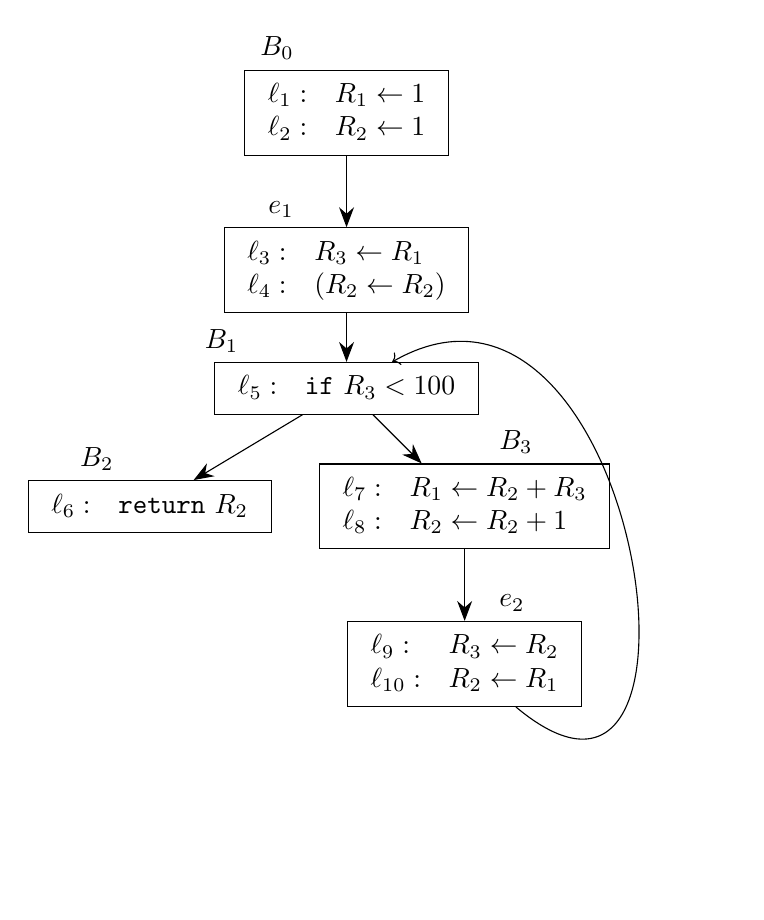
\begin{tikzpicture}
\node[draw,label={135:$B_0$}] (N1) at (0,0) {$\begin{array}{ll}
    \ell_1: & R_1\leftarrow 1\\
    \ell_2: & R_2\leftarrow 1\end{array}$};
\node[draw,label={135:$e_1$}] (N12) at (0,-2) {$\begin{array}{ll}
    \ell_3: & R_3\leftarrow R_1\\
    \ell_4: & (R_2\leftarrow R_2)
\end{array}$};
\node[draw,label={165:$B_1$}] (N2) at (0,-3.5) {$\begin{array}{ll}
    \ell_5: & \texttt{if}\ R_3<100
\end{array}$};
\node[draw,label={135:$B_2$}] (N3) at (-2.5,-5) {$\begin{array}{ll}
    \ell_6: & \texttt{return}\ R_2
\end{array}$};
\node[draw,label={60:$B_3$}] (N4) at (1.5,-5) {$\begin{array}{ll}
    \ell_7: & R_1\leftarrow R_2+R_3\\
    \ell_8: & R_2\leftarrow R_2+1\end{array}$};
\node[draw,label={60:$e_2$}] (N42) at (1.5,-7) {$\begin{array}{ll}
    \ell_9: & R_3\leftarrow R_2\\
    \ell_{10}: & R_2\leftarrow R_1
\end{array}$};
\path[-{Stealth[scale=1.5]}] (N1) edge (N12) (N12) edge (N2) (N2) edge (N3) (N2) edge (N4) (N4) edge (N42);
\path[->] (N42) edge [out=320,in=30,looseness=2] (N2);
\end{tikzpicture}

\end{document}